 \documentclass[book.tex]{subfiles}
\begin{document}

\section{Smooth scrolling on EGA}
\label{section:adaptive_tile_refresh}
Performing a full-screen redraw per frame would kill the CPU, as it would require updating every pixel on all four EGA planes. Achieving a 60Hz frame rate while refreshing the entire screen is impossible under these constraints. If we were to run the following code, which simply fills all memory banks, it would run at 5 frames per seconds.\\

\par
\begin{minipage}{\textwidth}
  \lstinputlisting[language=C]{code/write_ega.c}
  \end{minipage}
  \label{ega_write}

\bigskip
\par
\begin{fancyquotes}
Clearly, there is a whole world of awesome things there that we just couldn't do on the PC...\\

\par 
You can just redraw the whole screen, but then it turns out...\\
\par
Well, you're going five frames a second.\\

\par
\textbf{John Carmack\protect\footnotemark}
\end{fancyquotes}\\
\addtocounter{footnote}{-1}
\stepcounter{footnote}
\footnotetext{Interview with Lex Fridman in 2022, this quote is around 1h:41m.}

\pagebreak
So, how did they create a smooth scrolling game with these limitations? The solution was twofold:
\begin{itemize}
  \item Utilizing specific EGA hardware tricks
  \item Updating only the portion of the screen that has changed
\end{itemize}

\par
Each method is described in detail in the following sections.

\subsection{EGA Virtual Screen and Pel Panning}
\label{section:EGA_virtual_screen}
The EGA card adds a powerful approach to linear addressing: the logical width of the virtual screen in VRAM does not need to match the physical screen display width. A programmer can define a virtual screen width of up to 4096 pixels and use the physical screen as a window onto any part of the virtual screen. What's more, the virtual screen's logical height can extend up to the total VRAM capacity. The code below demonstrates how to set a custom logical width.\\

\begin{minipage}{\textwidth}
  \lstinputlisting[language=C]{code/SCREEN_WIDTH.ASM}
  \end{minipage}
  \label{ega_pel_pan}
  
\par
The displayed area of the virtual screen at any time is determined by setting the display memory address for fetching video data, configured via the CRTC Start Address register. The default address is \cw{A000:0000h}, though the offset can be adjusted to any other address.\\


\begin{minipage}{\textwidth}
  \lstinputlisting[language=C]{code/EGA_SET_ADDRESS.ASM}
  \end{minipage}
  \label{ega_set_address}
  \par


\par
To pan down a scan line, it requires only to increase the CRTC start address by the logical width. Horizontal panning is achieved by incrementing the start address by one byte. In EGA's planar graphics modes, the eight bits in each video RAM byte correspond to eight consecutive on-screen pixels, meaning the screen can move horizontally in steps of 8 pixels. This is rather coarse and not really smooth horizontal scrolling. Fortunately, another EGA register addresses this limitation.\\

\begin{figure}[H]
\centering
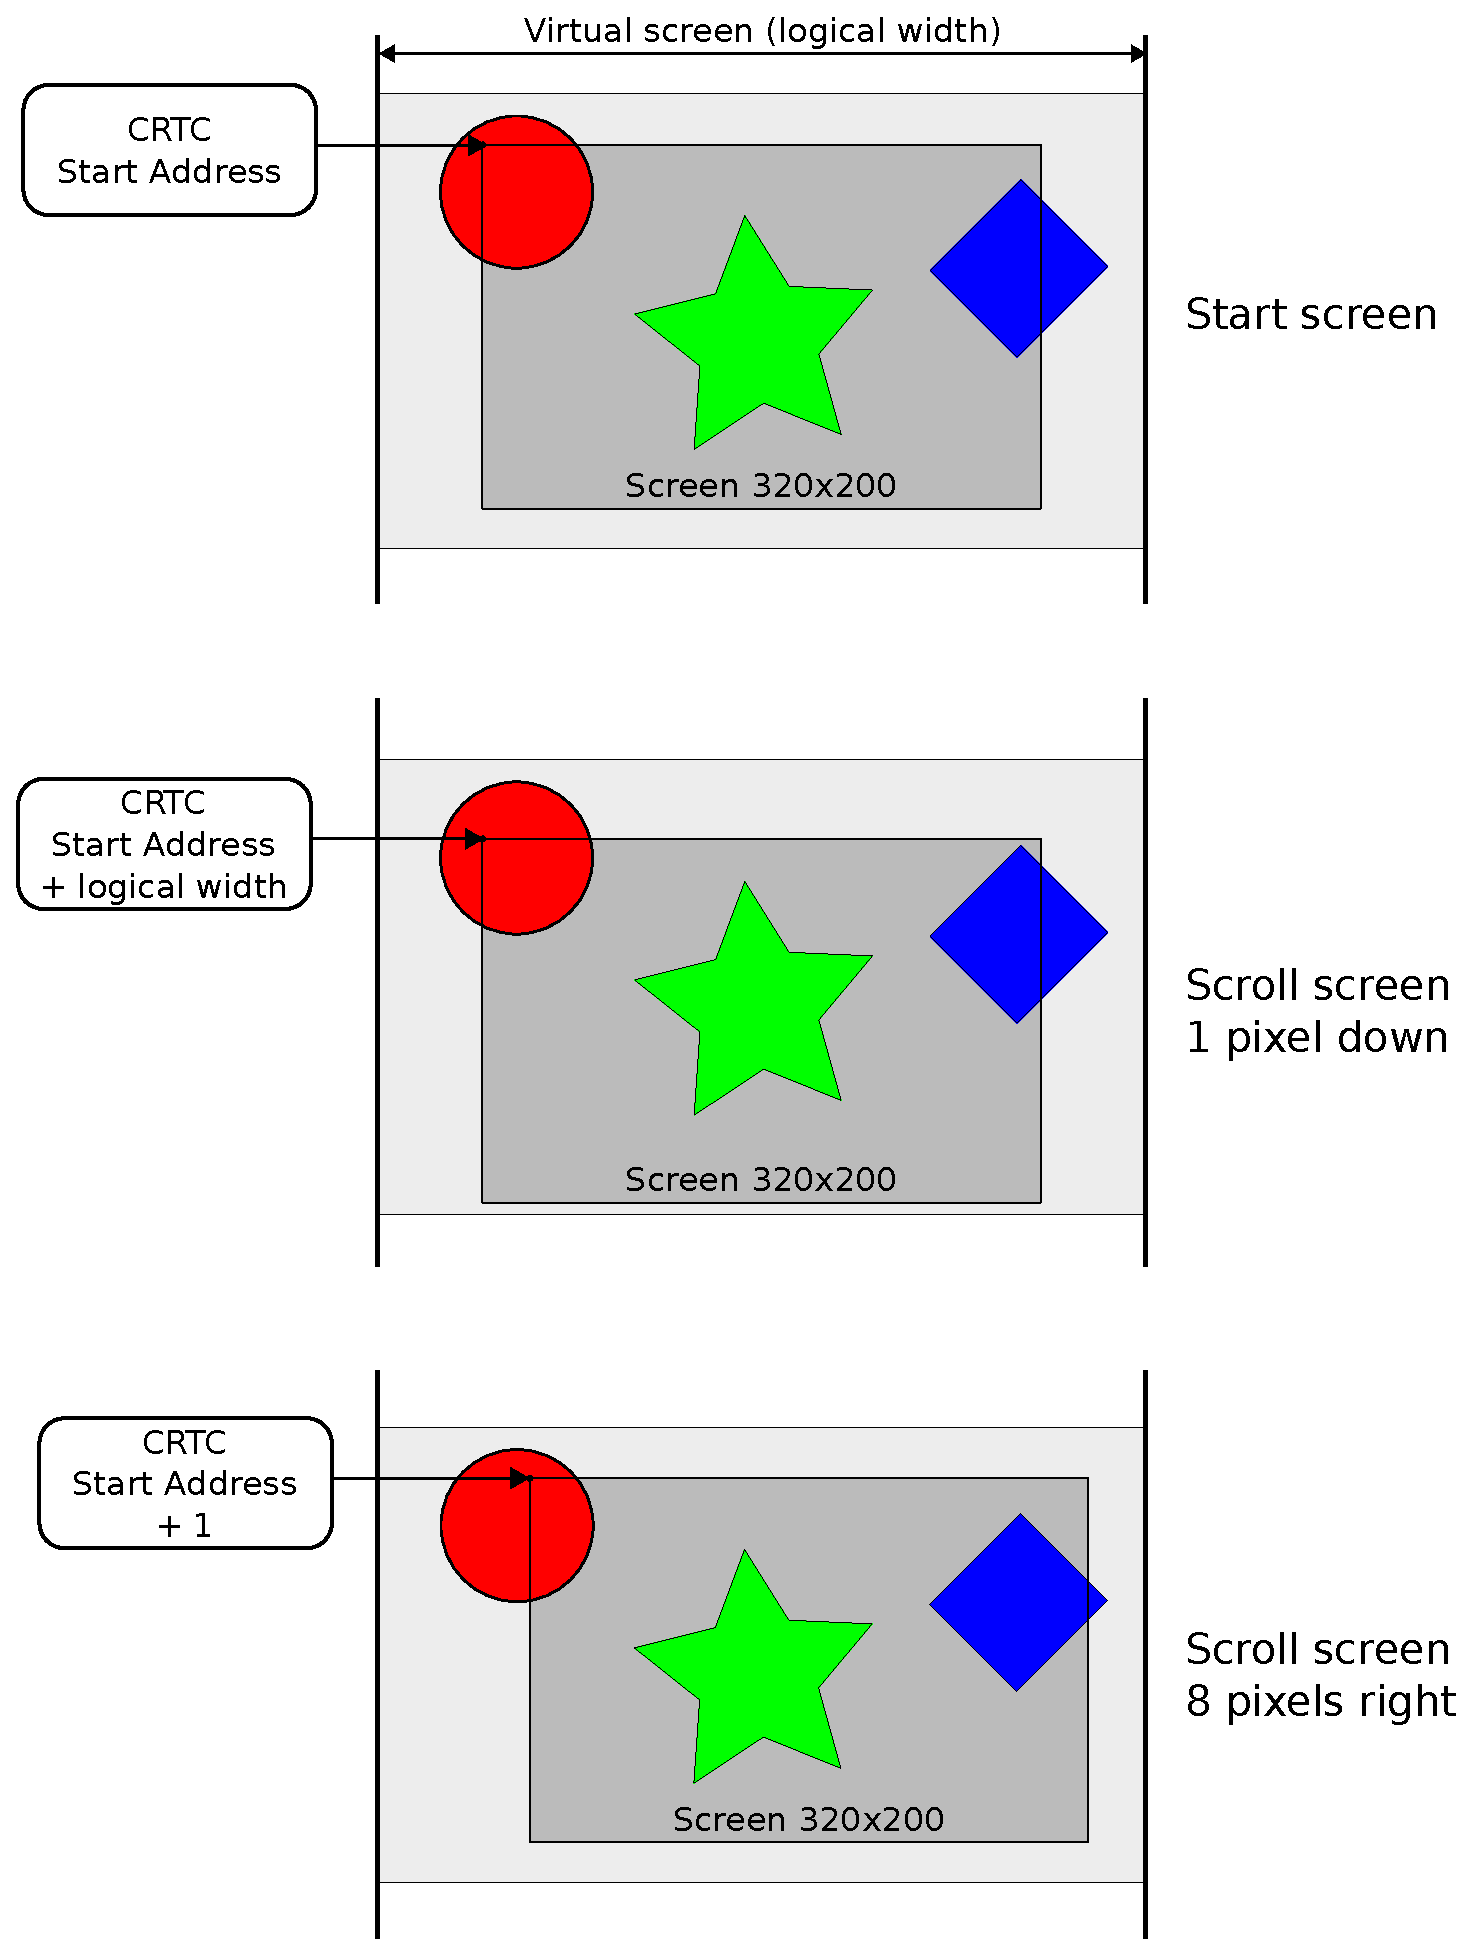
\includegraphics[width=1.0\textwidth]{imgs/drawings/virtual_screen.eps}
\caption{EGA screen scrolling by updating the CRTC Start Address.}
\label{fig:tile_refresh}
\end{figure}



\subsection{Horizontal Pel Panning}
Smooth horizontal pixel scrolling is managed by the "Horizontal Pel Panning" register in the Attribute Controller (ATC), allowing fine adjustment in 1-pixel increments up to 7 pixels to the left. \\

\par
However, programming the ATC requires attention: the ATC Index register only uses the lower five bits (bits 0-4) as its internal index. The next most significant bit, bit 5, controls the source of the video data send to the monitor by the EGA card. When bit 5 is set to 1, the output of the color palette controls the displayed pixels; this is normal operation. When bit 5 is 0, video data doesn't come from the color palette, and the screen becomes a solid color. To maintain normal video operation, bit 5 must be set to 1 by writing \cw{20h} to the register.\\

\begin{minipage}{\textwidth}
  \lstinputlisting[language=C]{code/EGA_PELPAN.ASM}
  \end{minipage}
  \label{ega_pel_pan}
 
\par
Smooth horizontal scrolling on EGA involves adjusting the CRTC Start Address alongside fine-tuning within an 8-pixel range using horizontal pel panning. The following steps accomplish this:
\begin{itemize}
  \item Calculate the panning offset in pixels for both \cw{x-} and \cw{y-}direction.
  \item Smooth y-panning is achieved by adding the \cw{(logical width *) y} to the CRTC start address.
  \item For coarse horizontal scrolling, increase the CRTC start address by \cw{x /8 } bytes.
  \item Fine horizontal adjustment is applied using \cw{(x \% 8)} to the horizontal pel panning register.
\end{itemize}


\begin{figure}[H]
\centering
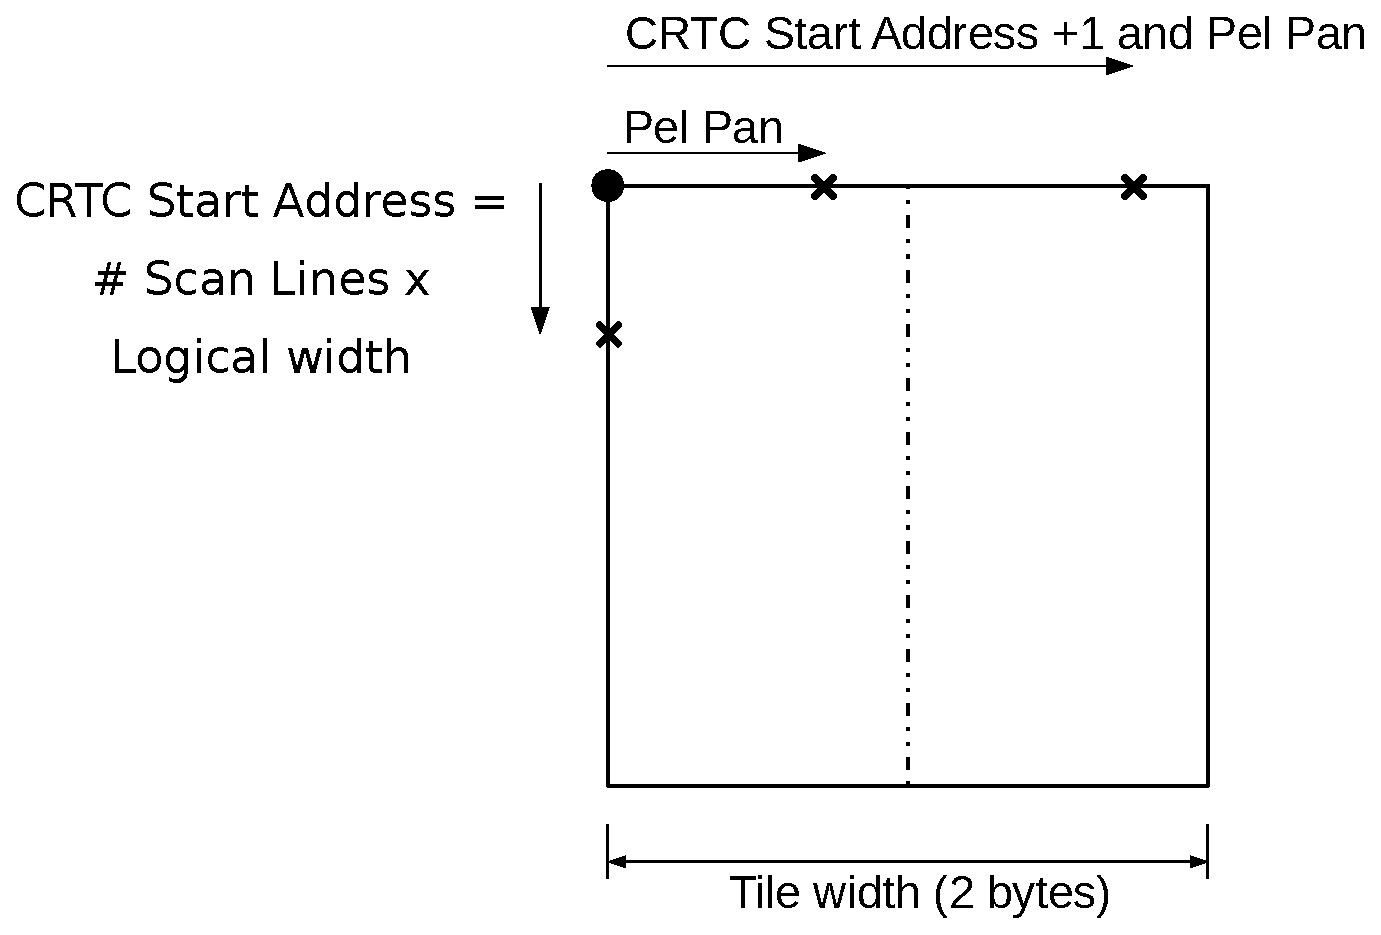
\includegraphics[width=0.55\textwidth]{imgs/drawings/Tile_Refresh.eps}
\caption{Smooth scrolling in EGA.}
\label{fig:tile_refresh}
\end{figure}


\section{Adaptive Tile Refreshment}
So far, we have built a virtual screen in VRAM allowing smooth one pixel moves in both axes using only EGA registers. However, once the screen edge is reached, a full-screen redraw would be too slow, causing a drop to 5 fps.\\


\begin{figure}[H]
\centering
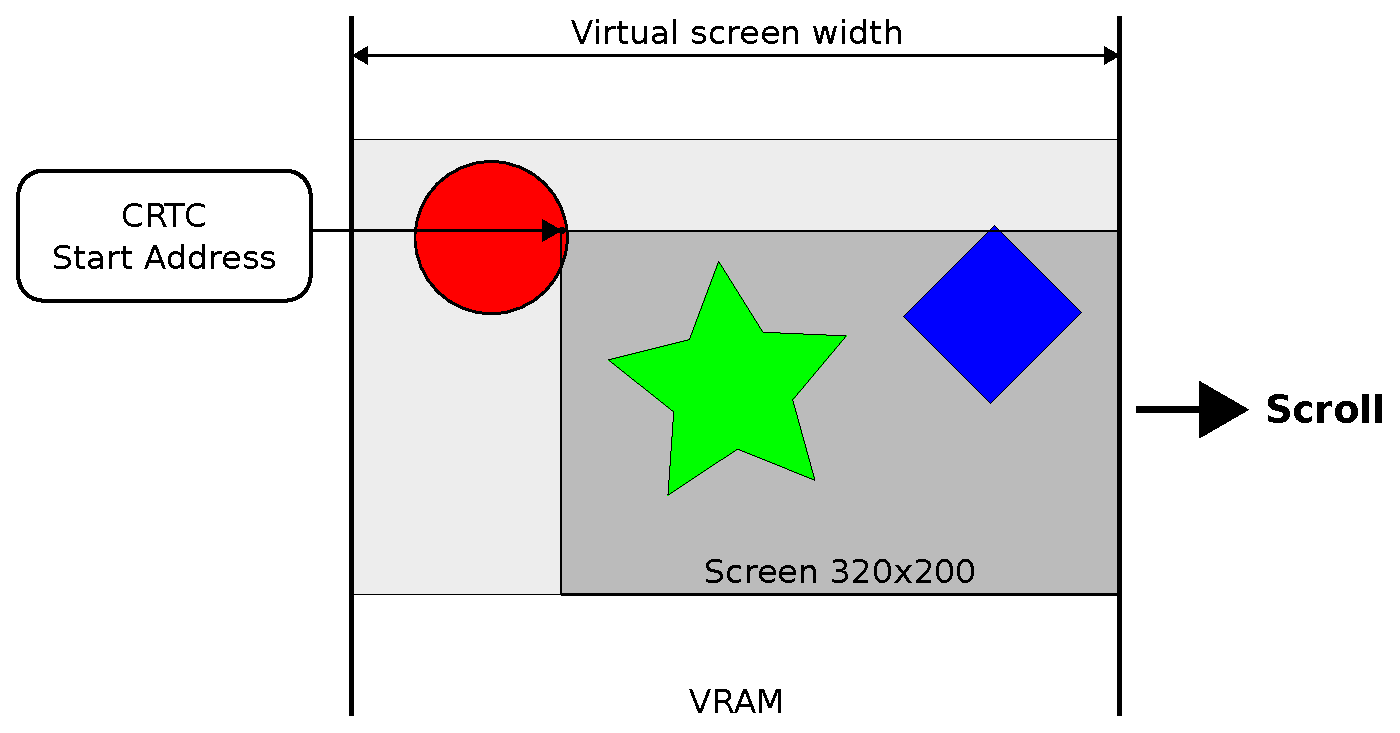
\includegraphics[width=0.8\textwidth]{imgs/drawings/screen_edge.eps}
\caption{Screen reaching the edge of virtual screen.}
\label{fig:screen_edge}
\end{figure}

\par
One option for screen refresh is to load the entire level into VRAM, setting the logical width to match the level width. By adjusting the CRTC Start Address and Horizontal Pel Panning registers, smooth scrolling can be achieved. However, loading the entire level requires far more VRAM than is available. The first level, \textit{Horsh Radish Hill}, is 136 tiles wide and 37 tiles high. Each tile is 128 bytes,  which means a total of 136 x 37 x 128 bytes = 644KB is required to store the entire level in VRAM. Since we only have 256KB available, this is not a feasible option.\\

\textbf{\underline{Trivia :}} At the time of writing this book, most video cards contain more than 1GB VRAM,  sufficient to store all Commander Keen levels at once in VRAM. \\

\par
To address this, John Carmack invented "Adaptive Tile Refresh" (ATR). The core idea is to refresh only those areas of the screen that need to change. \\

\par
Let's look at \textit{Commander Keen 1: Marooned on Mars} in Figure \ref{fig:keen_difference}. This is the first level of Marooned, immediately to the right of the crashed Bean-with-Bacon Megarocket. The first figure is the start of the level, the second figure is after Keen has scrolled one tile (16 pixels) to the right through the world. They look almost identical to the naked eye, don't they? \\

\par
Now, if we perform a difference on both images, you can see which tiles need to be changed upon screen refresh. The trick behind the scrolling is to only redraw tiles that actually changed after panning 16 pixels (one tile). For matching tiles there is nothing to do and they are skipped entirely. In Figure 4.21, there are large swathes of constant background tiles. In total, only 69 tiles out of the 260 tiles need to be refreshed, which is 27\% of the screen!\\

\par
This is also the part where the game designers Tom Hall and Jogn Romero had to help the engine. Smooth scrolling is inversely proportional to the number of tiles to redraw. A checkerboard tile pattern basically means a full-screen redraw and would kill the CPU. So to avoid costly "jolts", the game designers built tile maps with a lot of reperating tiles. \\



\pagebreak
\begin{figure}[H] 
  \centering 
  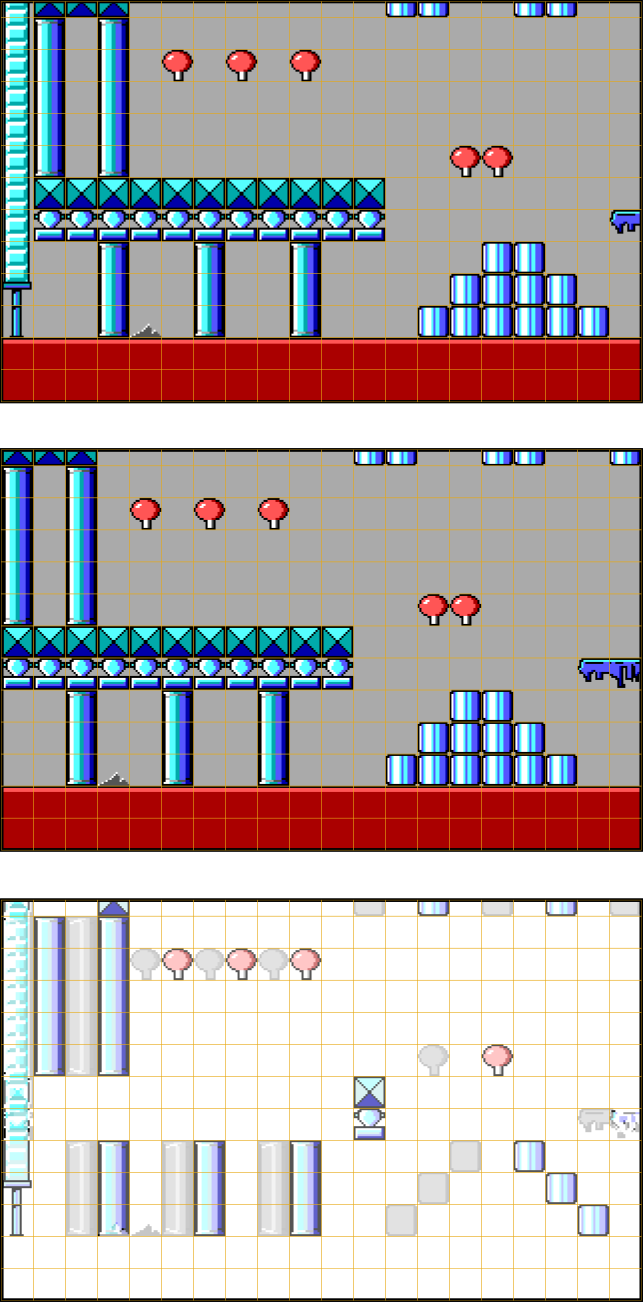
\includegraphics[width=.66\textwidth]{screenshots_300dpi/game/keen-ATR-diff.png}
  \caption{Start of the world, moved one tile to the right and difference.}
  \label{fig:keen_difference}
\end{figure}
\pagebreak

\subsection{Adaptive tile refreshment in Commander Keen 1-3}
This section explains how ATR is working for the first three episodes of Commander Keen. Since there is no source code released for these episodes, ATR will be explained without code examples. The later versions of Commander Keen, including Keen Dreams, used a different, improved engine which will be explained in the next section\footnote{https://retrocomputing.stackexchange.com/questions/22175/what-is-adaptive-tile-refresh-in-the-context-of-commander-keen}.\\


\par
The EGA screen in mode \cw{0xD} has a resolution of 320x200 pixels, or 40x200 bytes. Let's extend the height by 8 bytes to have a height of 208 pixels, so the screen fits nicely in 20x13 tiles. By making the virtual screen one tile higher and one wider on each side of the screen, the engine can scroll up to 16 pixels to any direction of the screen without any tile refresh, by simply adjusting the CRTC Start Address and Pel Pan registers.\\


\begin{figure}[H]
\centering
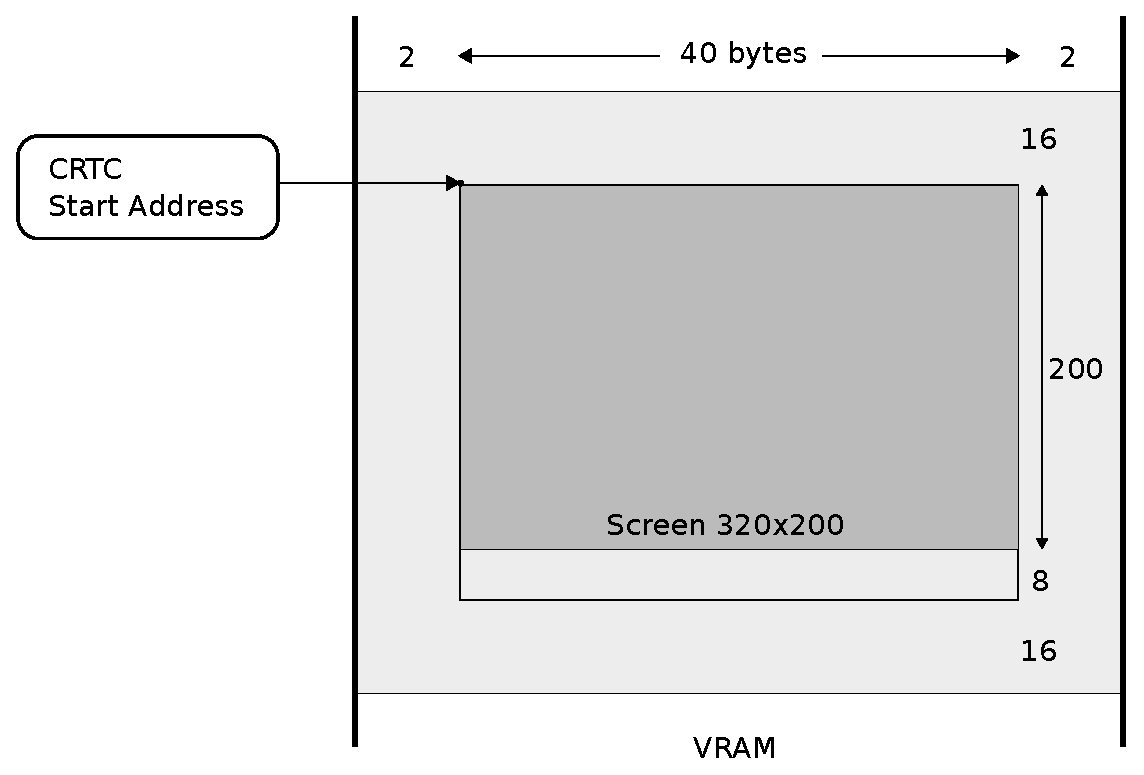
\includegraphics[width=0.8\textwidth]{imgs/drawings/ATR_virtual_screen.eps}
\label{fig:atr_virtual screen}
\end{figure}

 
 
Now, let's have a closer look at the EGA VRAM setup. The video memory is organized into three virtual screens:
\begin{itemize}
\item Page 0 and 1, which are used to switch between buffer and visible screen. The idea between two pages (double buffer) is that the code can draw in the second buffer while the first buffer is being shown on screen, which is then switched out during screen refresh. This ensures that no frame is ever displayed mid-drawing, which yields smooth, flicker-free animation.
\item A master page containing a static page, which is copied to the buffer screen when performing the screen refresh.
\end{itemize}



\par
Each virtual screen has a size of 44*240*4=42,420 bytes. So within a 256KB EGA card there is enough VRAM available to keep all three virtual screens in memory. The page that is displayed on screen is selected by setting the CRTC Start Address register at which to begin fetching video data.\\



\begin{figure}[H]
\centering
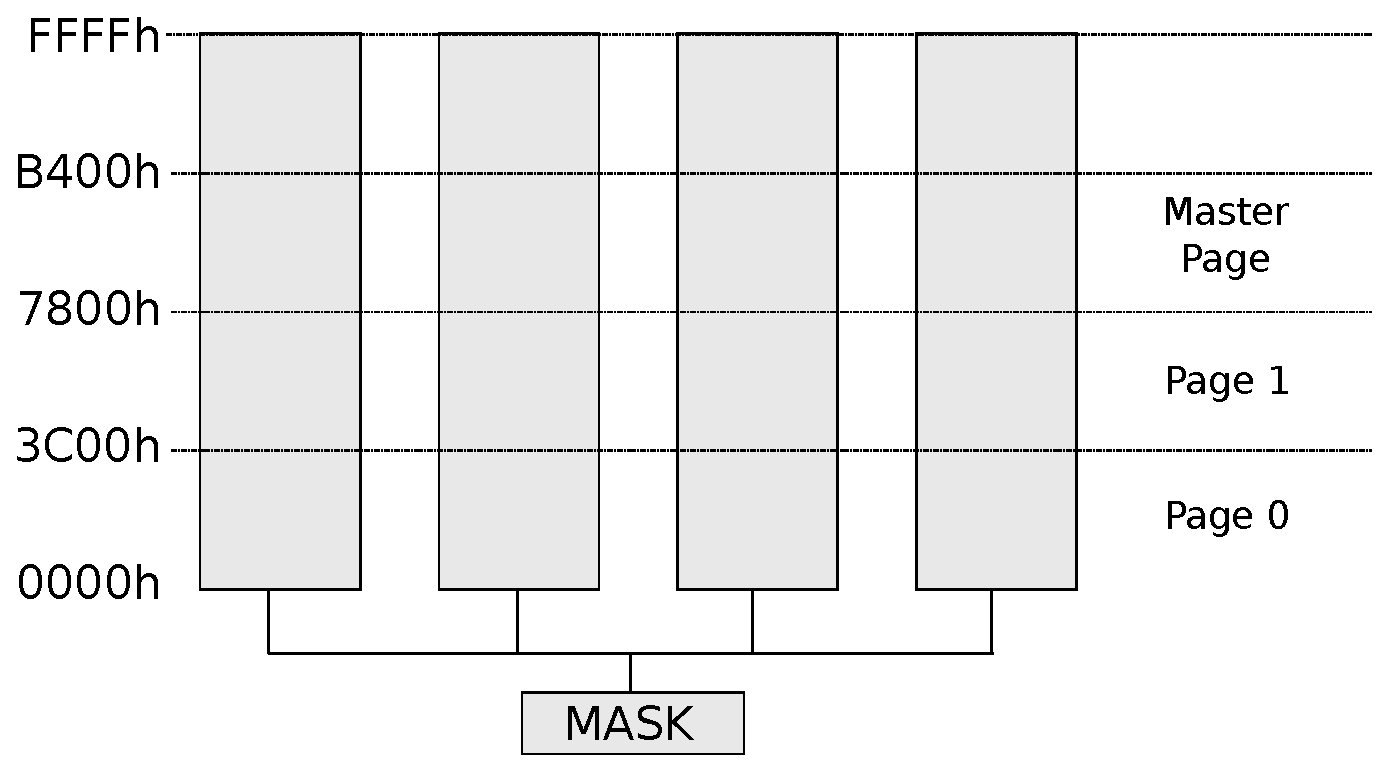
\includegraphics[width=\textwidth]{imgs/drawings/ega_ram_architecture.eps}
\caption{Virtual screen layout on EGA card.}
\label{fig:ega_ram_arch}
\end{figure}

\par
For both the buffer and visible screen a tile array is created to maintain which tiles are changed since last refresh.\\


\par
\begin{minipage}{\textwidth}
  \lstinputlisting[language=C]{code/tile_index_array.c}
  \end{minipage}
  \label{ega_refresh}
  \par

Steps to refresh the screen are as follows:
\begin{enumerate}
\item Check if the player has moved one tile in any direction.
\item Identify changed tiles and copy these to the master page, marking them in both tile arrays. 
\item Refresh the buffer page by copying marked tiles from the master page.
\item Switch the view and buffer pages by adjusting the CRTC Start Address and Pel Panning registers.
\end{enumerate}


Ignoring sprites for now, the following steps illustrate these stages. In the next four screenshots, we take you step-by-step through each of the stages. The player has reached the edge of the virtual screen and moves further to the right.\\

 
\begin{figure}[H]
\centering
 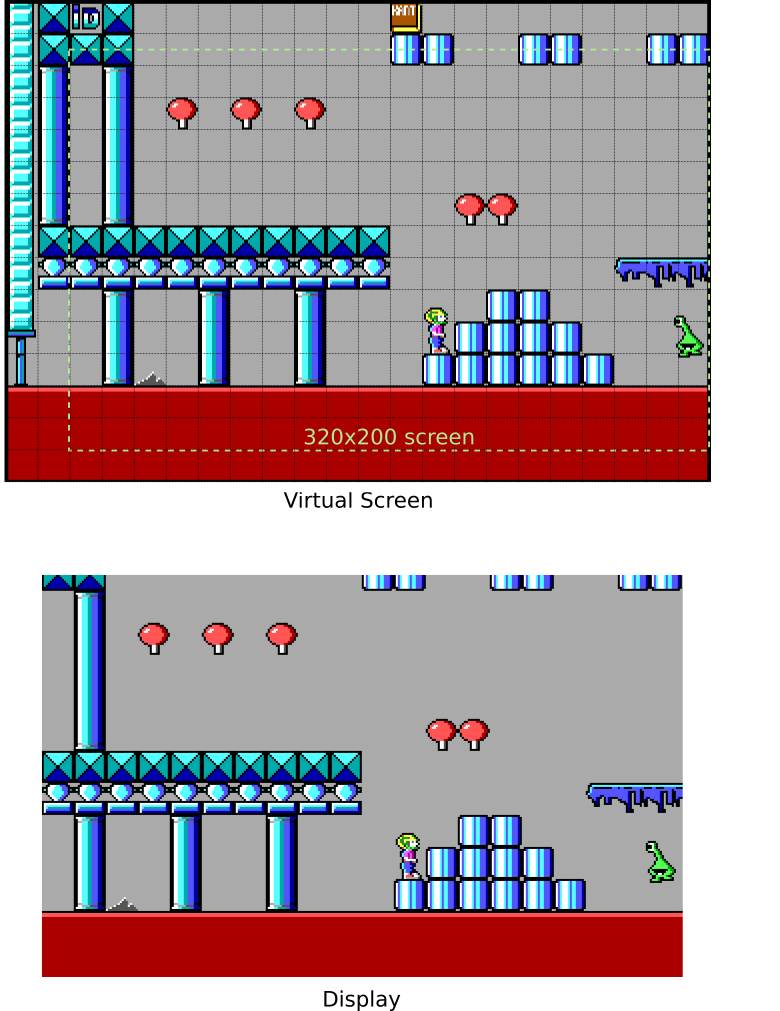
\includegraphics[width=0.85\textwidth]{screenshots_300dpi/game/Keen_ATR_1-3_a.png}
 \caption{Start: Reach the end of the virtual screen.}
 \label{fig:kc1_3_start}
\end{figure}

\pagebreak
The engine keeps track of which tile numbers are part of the virtual screen. Since the engine only refresh the screen at tile size granularity, it can determine extremely fast what has changed on the screen by comparing tile numbers. If the tile number has changed, the tile is updated by copying tiles from RAM into the VRAM master page. The changed tiles are marked with a '1' in both tile arrays, meaning it needs to be updated upon next refresh.

\begin{figure}[H]
\centering
 \fullimage{/game/Keen_ATR_1-3_step1.png}
 \caption{Update tiles in master page and update both tile arrays.}
 \label{fig:kc1_3_step1}
\end{figure}

\pagebreak
The next step is to scan all tiles in buffer tile array (array 1) and for each tile marked '1', copy the corresponding tile from master to virtual page 1 page.\\

\begin{figure}[H]
\centering
 \fullimage{/game/Keen_ATR_1-3_step2.png}
 \caption{Copy changes tiles from virtual master page to page 1.}
 \label{fig:kc1_3_step2}
\end{figure}


\pagebreak
In the final step, point the visible screen to virtual page 1 by updating the CRTC start address. Finally, tile array 1 is cleared to '0'. Now the first step is repeated, but this time virtual page 0 acts as the buffer screen. Note that after swapping, tile array 0 keeps marked tiles from last update. This makes sense, as the current buffer page is not yet refreshed since it was displayed in the previous refresh cycle. 

\begin{figure}[H]
\centering
 \fullimage{/game/Keen_ATR_1-3_step3.png}
 \caption{Update CRTC Start Address to virtual page 1 and empty tile array 1.}
 \label{fig:kc1_3_step2}
\end{figure}

\pagebreak

Now the buffer is refreshed and the CRTC address is updated, the final step is fine adjustment using the Pel Panning register.
\begin{figure}[H]
\centering
 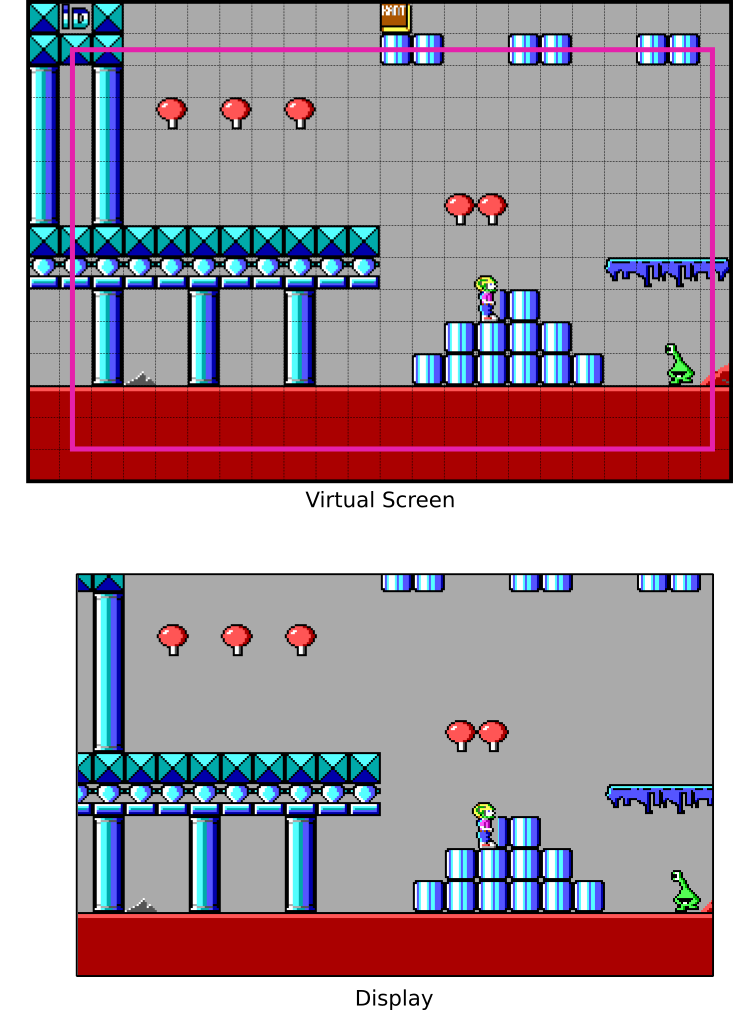
\includegraphics[width=0.85\textwidth]{screenshots_300dpi/game/Keen_ATR_1-3_b.png}
 \caption{Screen is refreshed and scrolled to the right.}
 \label{fig:kc1_3_start}
\end{figure}



\subsection{Wrap around the EGA Memory}
\label{section:wrap_ega_memory}
\label{section:optimize_tile}
John Carmack explored what would happen if you push the virtual screen over the 64kB border (address \cw{0xFFFF}) in video memory. It turned out that the EGA continues the virtual screen at \cw{0x0000}. This means you could wrap the virtual screen around  the EGA memory and only need to add a stroke of tiles on one of the edges when Commander Keen moves more than 16 pixels.\\
\par
\begin{figure}[H]
  \centering
  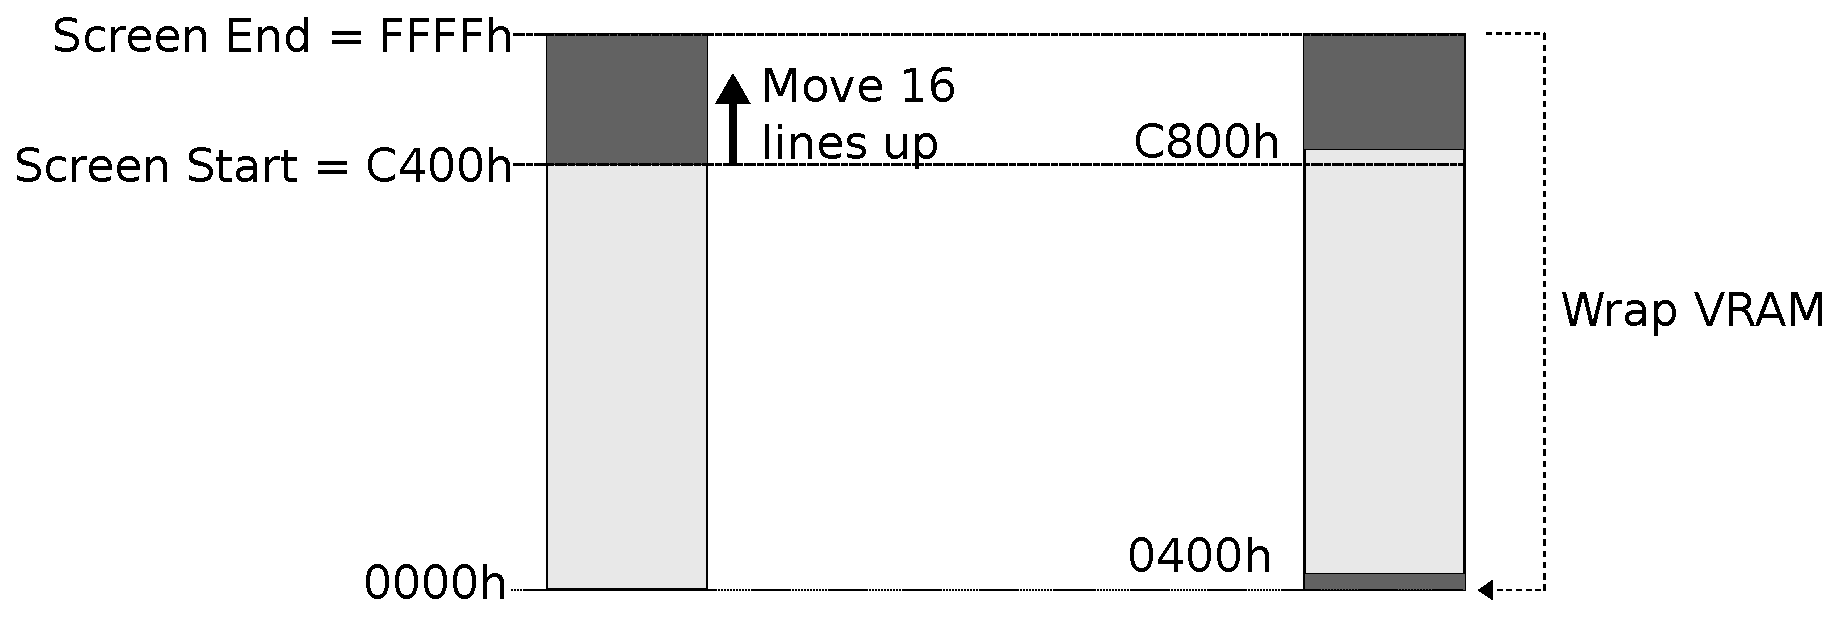
\includegraphics[width=0.95\textwidth]{imgs/drawings/ega_wrapping.eps}
  \label{fig:ega_wrapping}
  \caption{Wrap virtual screen around the EGA memory}
\end{figure}
 
\par
\begin{fancyquotes}
I finally asked what actually happens if you just go off the edge [OF THE VRAM]?\\

If you take your [CRTC] start and you say OK, I can move over and I get to what should be the bottom of the memory window. [...] What happens if I start at 0xFFFE at the very end of the 64k block? It turns out it just wraps back around to the top of the block.\\

I'm like oh well this makes everything easy. You can just scroll the screen everywhere and all you have to draw is just one new line of tiles.\\

It just works. We no longer had the problem of having fields of similar colors. It doesn't matter what you're doing, you could be having a completely unique world and you're just drawing the new strip.\\
\par
\textbf{John Carmack\protect\footnotemark}
\end{fancyquotes}\\
\addtocounter{footnote}{-1}
\stepcounter{footnote}
\footnotetext{An explanation further elaborated during the same interview with Lex Fridman in 2022.}

\par
There was however an issue with the introduction of Super VGA cards, which had typically more than 256kB RAM\footnote{In 1989 the VESA consortium standardized an API to use Super VGA modes in a generic way. One of the first modes was 640x480 at 256 colors requiring at least 256kB RAM, which from a hardware constraint resulted in 512kB.}. This resulted in crippled backwards compatibility and the wrapping around \cw{0xFFFF} did not work anymore on these cards. \\
\par
There is an easy solution to resolve this issue. As you can see in Figure \ref{fig:ega_ram_arch} on page \pageref{fig:ega_ram_arch}, the space between \cw{0xB400} and \cw{0xFFFF} is not used and contains enough space for another virtual screen. In case the start address is between \cw{0xC400} and \cw{0xFFFF} the corresponding screen is copied to the opposite end of the buffer, as illustrated in Figure \ref{fig:page_wrapping}.\\

\par

\begin{fancyquotes}
I was in a tough position. Do I have to track every single one of these [SUPER VGA CARDS] and it was a madhouse back then with 20 different video card vendors with all slightly different implementations of their non-standard functionality. Either I needed to natively program all of the cards or I kind of punt. I took the easy solution of when you finally did run to the edge of the screen I accepted a hitch and just copied the whole screen up.\\
\par
\textbf{John Carmack\protect\footnotemark}
\end{fancyquotes}\\
\addtocounter{footnote}{-1}
\stepcounter{footnote}
\footnotetext{And again the same interview with Lex Fridman in 2022.}

\par 
\begin{figure}[H]
\centering 
\begin{subfigure}{.5\textwidth}
  \centering
  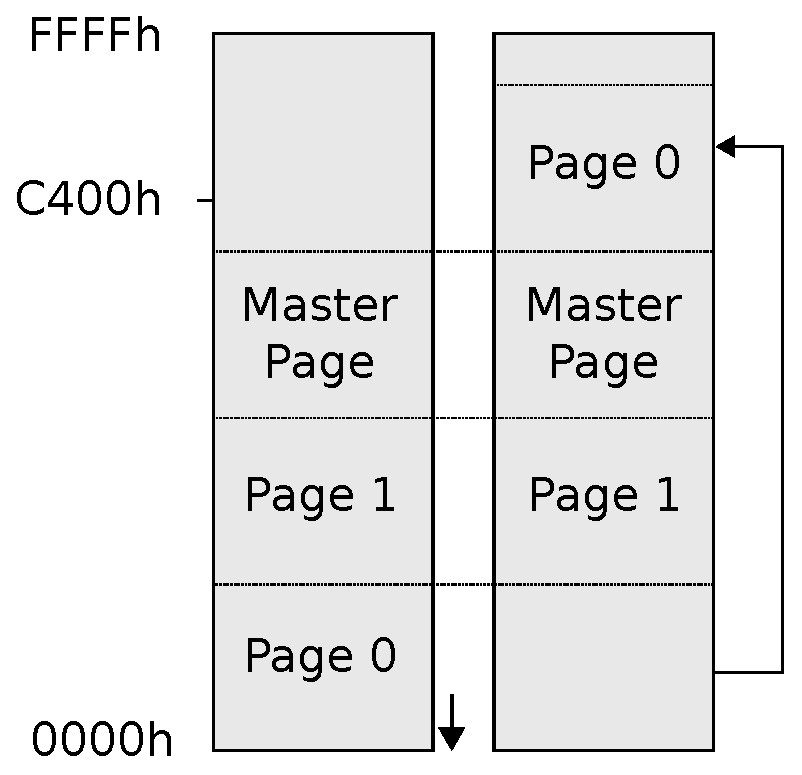
\includegraphics[width=.8\textwidth]{imgs/drawings/Page_down_switch.eps}
  \caption*{Copy Page 0 on top of Master Page.}
  \label{fig:page0_down}
\end{subfigure}%
\begin{subfigure}{.5\textwidth}
  \centering
  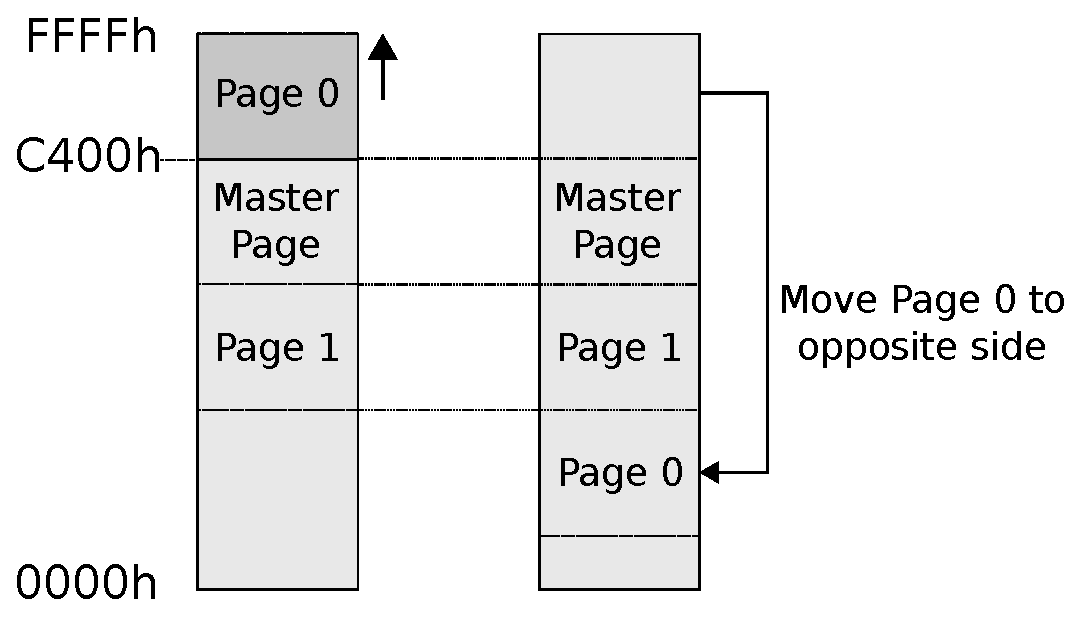
\includegraphics[width=.8\textwidth]{imgs/drawings/Page_up_switch.eps}
    \caption*{Copy Page 0 below Page 1. }
  \label{fig:page0_up}
\end{subfigure}
\caption{Move screen to opposite end of VRAM buffer}
\label{fig:page_wrapping}
\end{figure}



\par
\begin{minipage}{\textwidth}
  \lstinputlisting[language=C]{code/wrap_page_buffer.c}
  \end{minipage}
  \label{ega_refresh}
  \par
As explained in Section \ref{section:ega_memmap} each pixel is encoded by four bits, which are spread across the four EGA banks. So how can we copy four VRAM planes fast enough, without noticing any performance hit? To copy eight pixels, byte-aligned, one would have to do four read and four writes.\\



But how can we copy four VRAM planes fast enough, without noticing any performance hit? As explained in Section 3.3.7 each pixel is encoded by four bits, which are spread across the four EGA banks. To copy eight pixels, byte-aligned, one would have to do four read and four writes.\\

\par
Having a closer look at the EGA card one notice there is a latch placed in front of the ALU, which can be re-purposed for the greater good. With a little creativity the ALU in front of each bank can be setup to use only the latch for writing\footnote{The mask trick is discussed in \textit{Game Engine Black Book: Wolfenstein 3D} for the VGA card. The trick is the same for the EGA card.}. With such a setup, upon doing one read, four latches are populated at once and four bytes in the bank are written with only one write to the RAM. Now it is possible to copy the entire buffer fast enough, without notifying any performance impact.\\ 

\par
 \begin{figure}[H]
\centering
 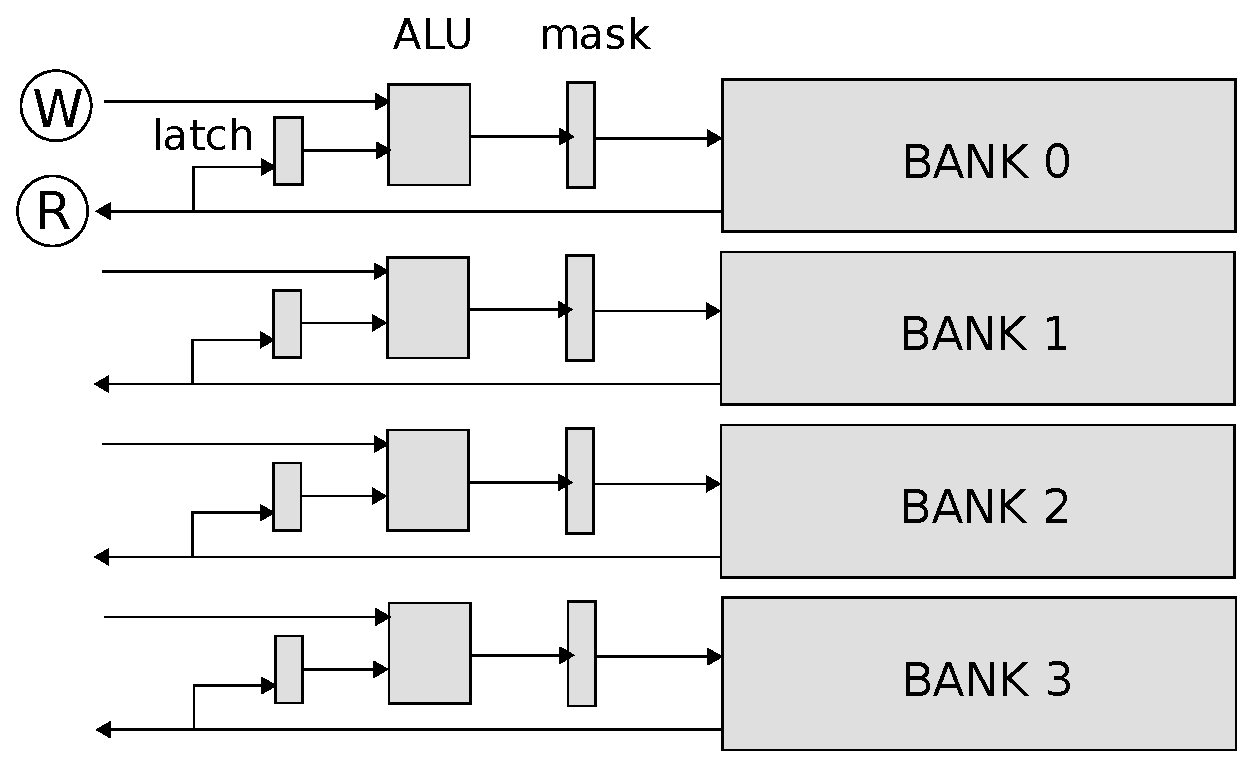
\includegraphics[width=\textwidth]{imgs/drawings/latches.eps}
 \caption{Latches memorize read operations from each bank. The memorized value can be used for later writes.}
 \end{figure}
 
 
\par
\begin{minipage}{\textwidth}
  \lstinputlisting[language=C]{code/EGA_LATCH_COPY.ASM}
  \end{minipage}
  \label{ega_latch_copy}


\subsection{Adaptive tile refreshment in Keen Dreams} 
\label{section:scroll_refresh_dreams}
The EGA memory wrapping results in an improved, more simplified Adaptive Tile Refreshment algorithm. First, a virtual screen and tile array is defined by making the display one tile taller and wider, creating what is known as the viewport. This allows the engine to scroll the display up to 16 pixels to the right and bottom without refreshing tiles, by simply adjusting the CRTC Start Address and Pel Pan register.\\

\par
An additional column is then added to the viewport to support horizontal scrolling. Finally, the tile array is further expanded to allow the entire viewport to move up to two tiles in any direction.\\


\begin{figure}[H]
\centering
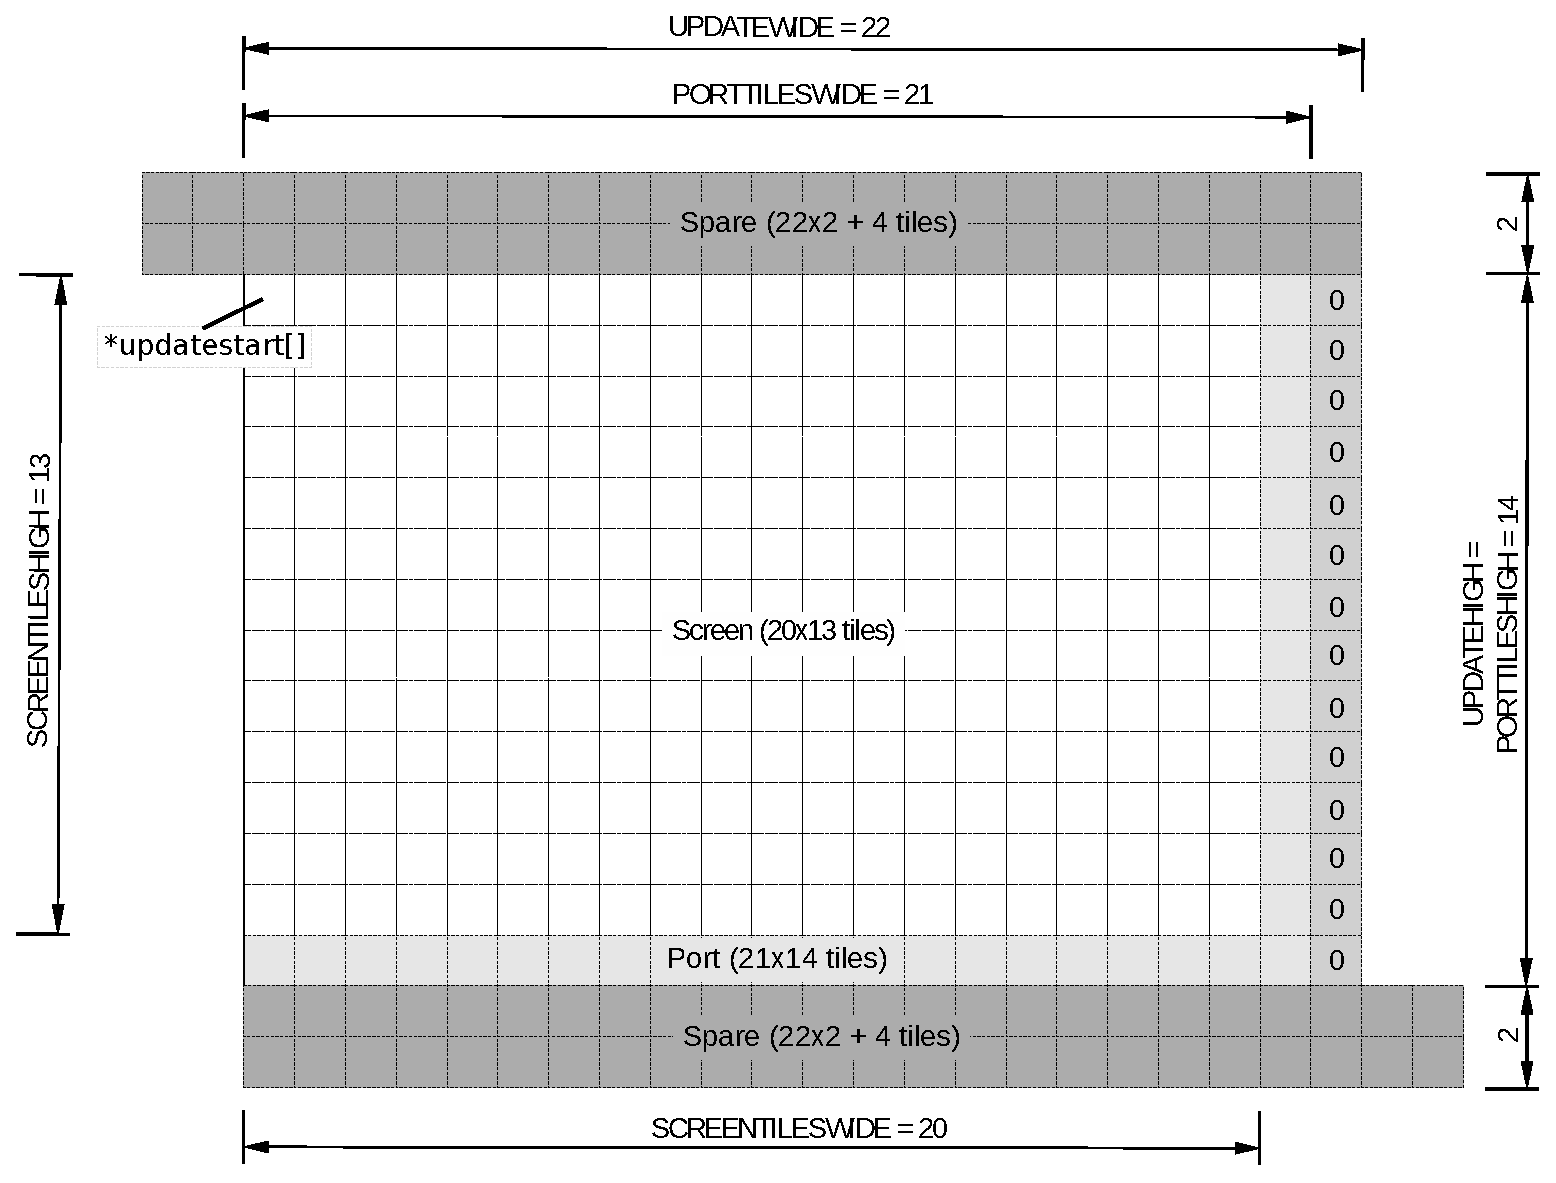
\includegraphics[width=\textwidth]{imgs/drawings/buffer_tile_layout.eps}
\caption{Tile array layout.}
\label{fig:screen_setup}
\end{figure}


\par
The full refresh cycle, including sprite updates, proceeds as follows:
\begin{enumerate}
  \item Verify if the player has moved one tile in any direction.
  \item Copy the new column or row of tiles to the master page, update both the tile array pointers, and mark the tiles in both arrays.
  \item Refresh the buffer page by scanning the tile index array. If a tile is marked, copy it from the master page to the buffer page.
  \item Iterate through the sprite removal list, copying the corresponding image block from the master page to the buffer page to clear the sprite.
  \item Iterate through the sprite list, copying each sprite image block to the buffer page.
  \item Switch the view and buffer pages by adjusting the CRTC Start Address and Pel Panning registers.
\end{enumerate}


\vspace{0.5cm}
\par
\begin{minipage}{\textwidth}
  \lstinputlisting[language=C]{code/refresh.c}
\end{minipage}
\label{state_type}


\pagebreak
Let's go over the refresh cycle step by step. At the start, all three virtual pages display the same viewport, with virtual page 0 currently shown on-screen. Both tile arrays are empty, meaning no tile updates are required in the next refresh cycle. The player has reached the edge of the virtual screen and moves further to the left. \\

\begin{figure}[H]
\centering
 \scaledimage{1.0}{/game/Keen_ATR_4-6_a.png}
 \caption{VRAM and tile arrays before scrolling to the left.}
 \label{fig:kc4_6_step0}
\end{figure}

\pagebreak
Both VRAM and tile array pointers shift left to introduce a new column of tiles. The VRAM pointer is lowered by 2 bytes (1 tile), and the tile array pointer is decreased by 1 byte.
A new column of tiles is copied from RAM to the master page, while the leftmost column in both tile arrays is marked with '1' to ensure it updates in the next refresh cycle. Animated tiles are then copied to the master page, and the corresponding tiles in the array are also marked with '1'.\\

\begin{figure}[H]
\centering
 \scaledimage{1.0}{/game/Keen_ATR_4-6_b.png}
 \caption{Update Virtual master with new left column and animated tiles.}
 \label{fig:kc4_6_step1}
\end{figure}

\pagebreak
Next, the engine scans all '1's and copies the corresponding tiles from the master to the buffer page. \\


\begin{figure}[H]
\centering
 \scaledimage{1.0}{/game/Keen_ATR_4-6_c.png}
 \caption{Copy changed tiles from master to buffer page.}
 \label{fig:kc4_6_step2}
\end{figure}

\pagebreak
Each sprite removed from the screen has its location and size stored in the sprite removal list, which removes the sprite by copying a specific section from the master screen to the virtual page. Tiles overlapping with the removal block are marked with a '2'.\\

\par
\begin{minipage}{\textwidth}
  \lstinputlisting[language=C]{code/erase_blocks_struct.c}
  \end{minipage}
  \label{block_removal}
\\
\par
\begin{minipage}{\textwidth}
  \lstinputlisting[language=C]{code/erase_blocks.c}
  \end{minipage}
  \label{block_removal}

\par
\textbf{\underline{Trivia :}} The '2' marking is nowhere used in the engine, most likely it is used in the original ATR algorithm.\\
  \par
  
\pagebreak
The final step in updating the buffer is copying sprites to their new locations, with each corresponding tile marked with a '3' in the tile array. 

\begin{figure}[H]
\centering
 \scaledimage{1.0}{/game/Keen_ATR_4-6_d.png}
 \caption{Removing and updating sprites to the buffer screen.}
 \label{fig:kc4_6_step4}
\end{figure}

\pagebreak
Once the buffer refresh is completed, the engine needs only to update the CRTC start address to virtual page 1. At this point, the visible tile array is emptied, and the pointer resets to its starting location. The new buffer array (virtual page 0) retains the marked tiles since this screen has not yet refreshed. At this point, the refresh cycle restarts, with virtual page 0 now functioning as the buffer. 

\begin{figure}[H]
\centering
 \scaledimage{0.99}{/game/Keen_ATR_4-6_e.png}
 \caption{Swap buffer and visible screen by updating CRTC start address.}
 \label{fig:kc4_6_step4}
\end{figure}

\pagebreak
The final step in scrolling is to adjust the horizontal fine-pixel alignment by setting the Pel Pan register. \textit{Et voil\`a}, the screen scrolls smoothly to the left. This scrolling process is significantly more efficient than the original ATR engine, resulting in only 8\% of tiles to be refreshed!\\

\begin{figure}[H]
\centering
\begin{subfigure}{.5\textwidth}
\centering
  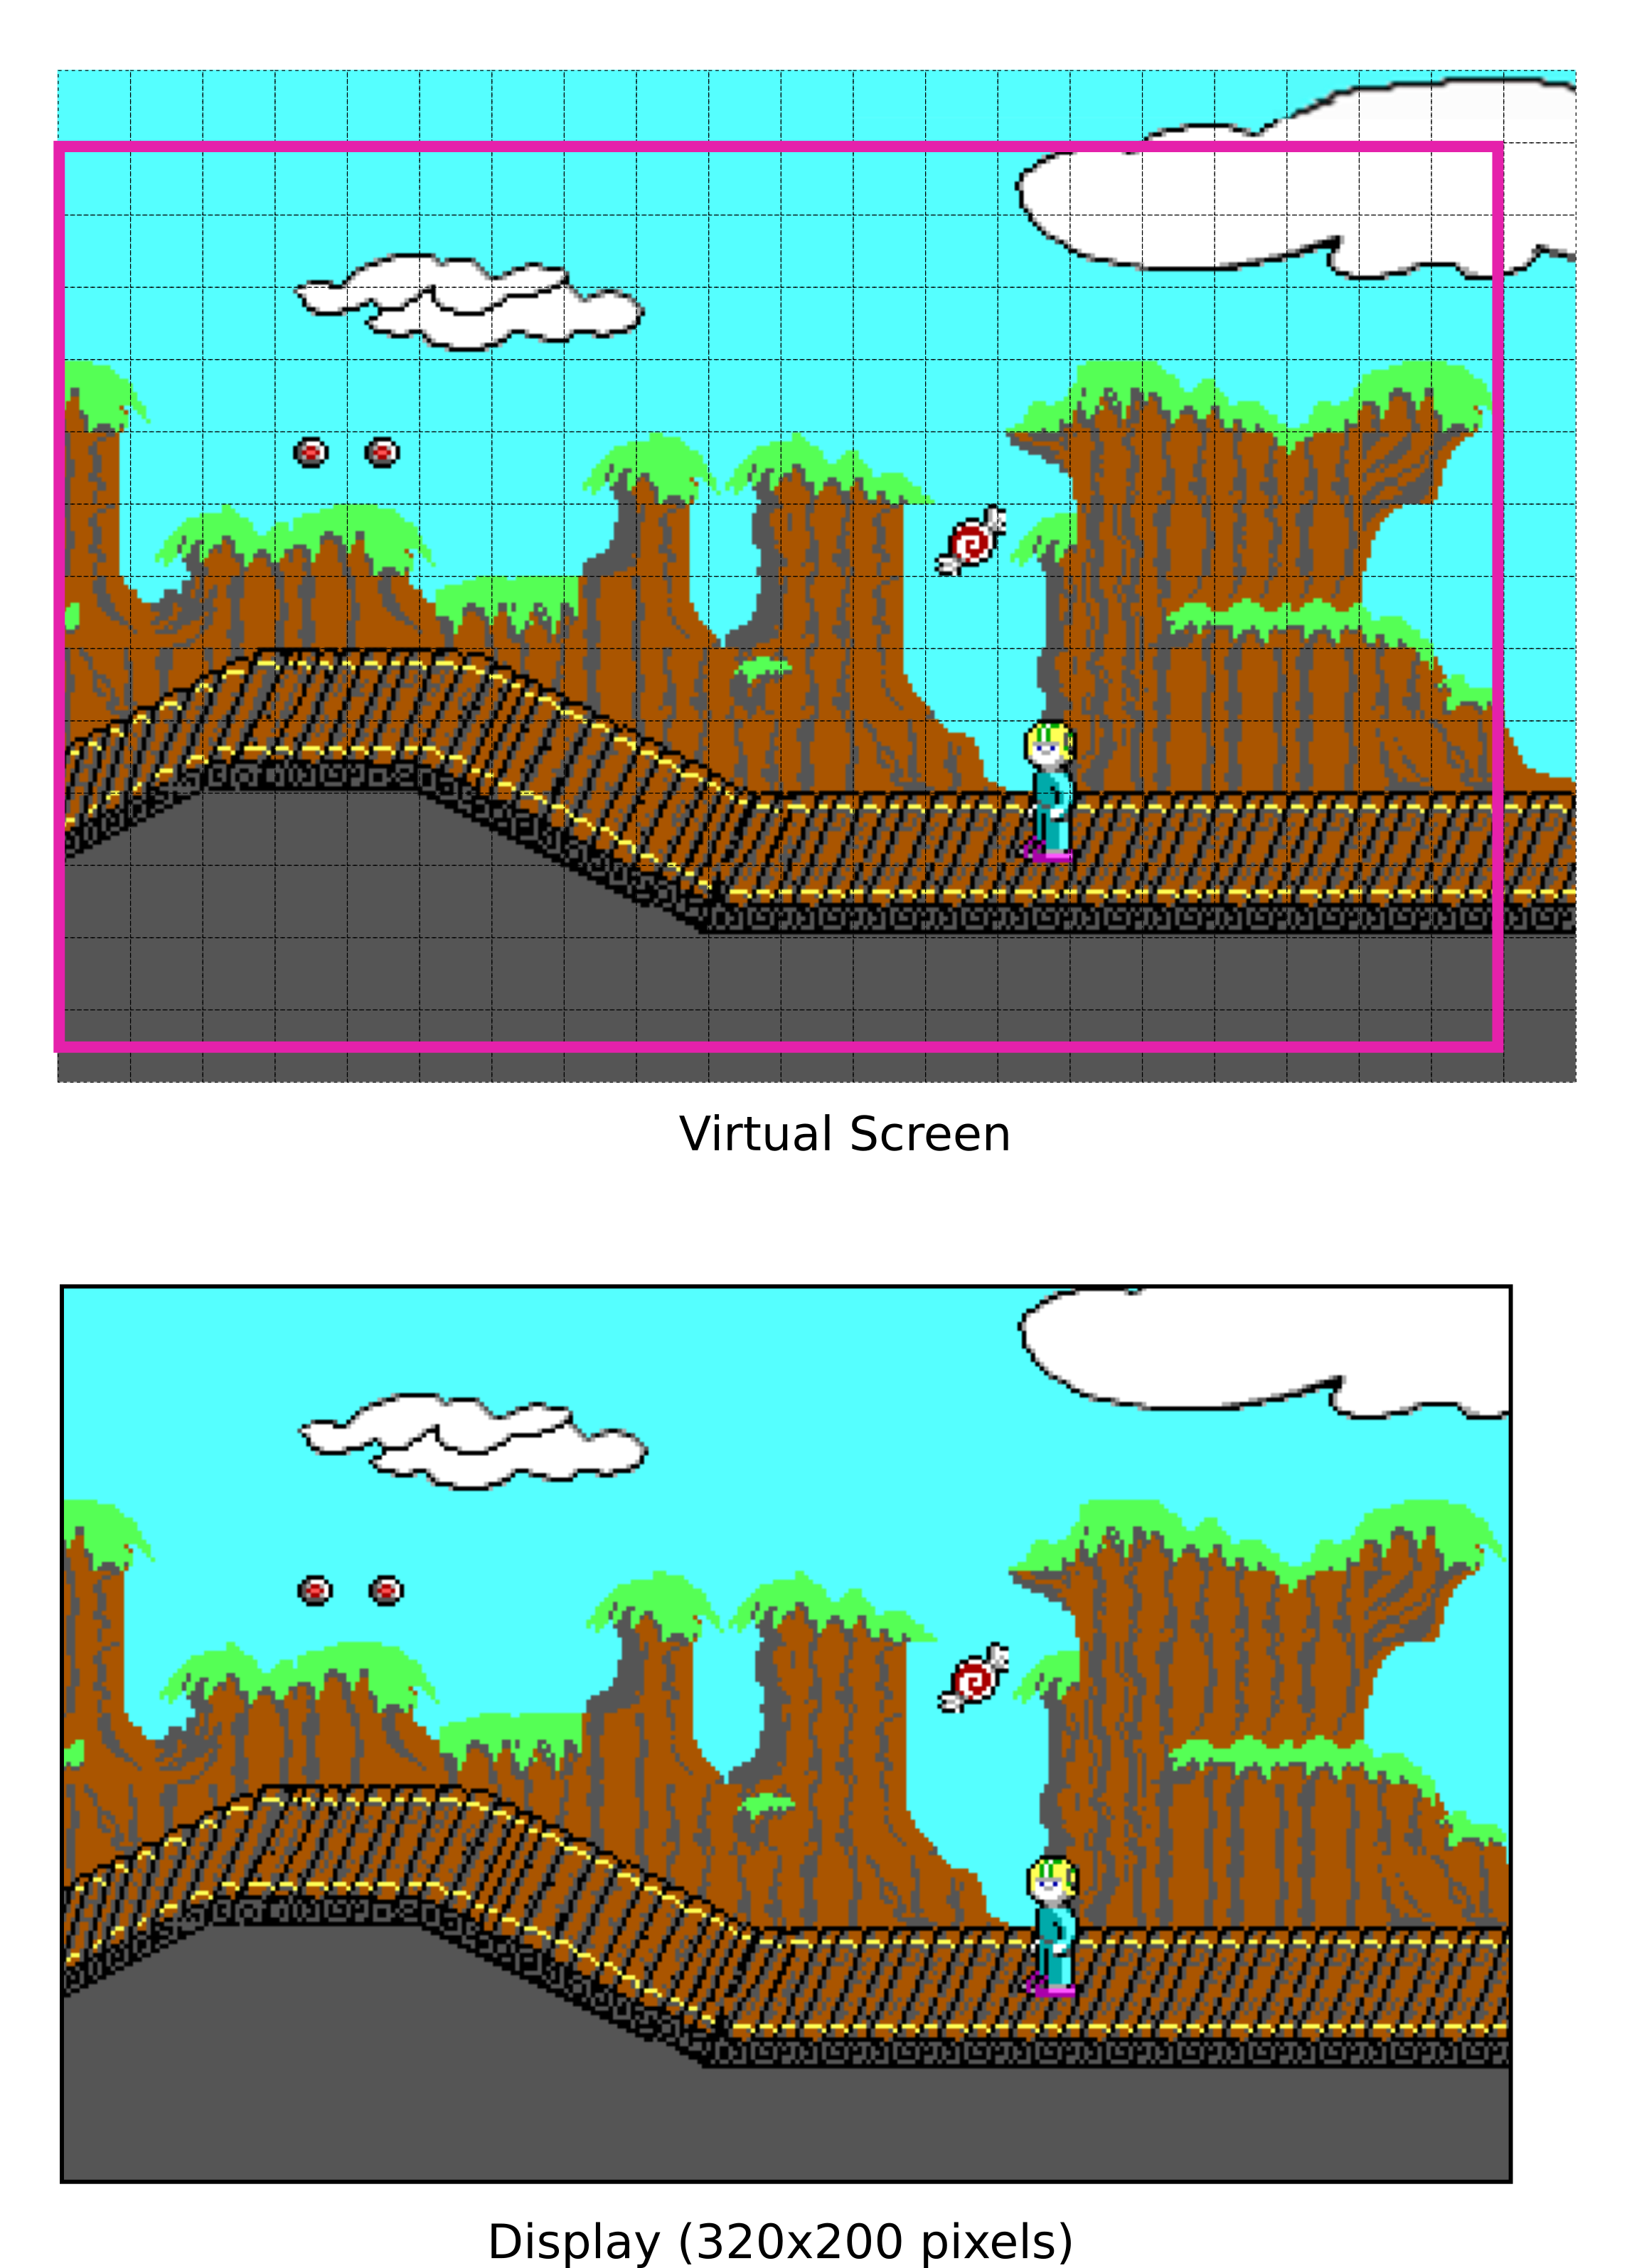
\includegraphics[width=.95\linewidth]{screenshots_300dpi/game/Scroll_KC4_6_1.png}
\end{subfigure}%
\begin{subfigure}{.5\textwidth}
\centering
  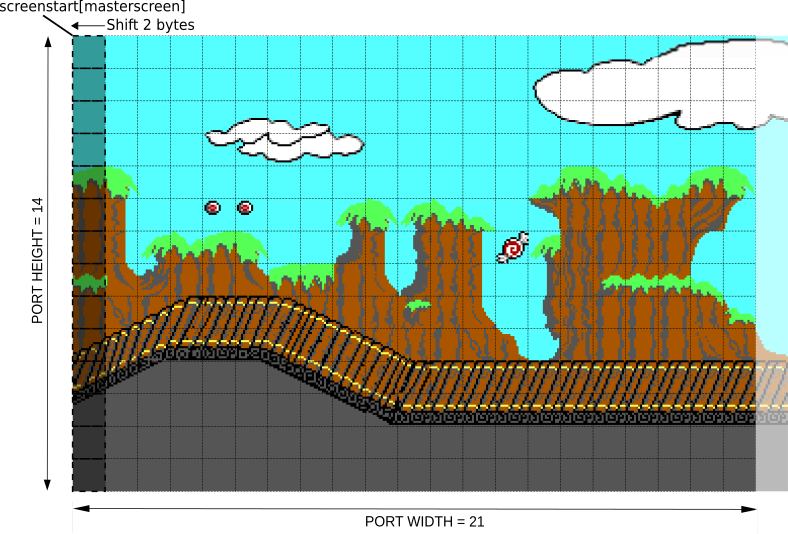
\includegraphics[width=.95\linewidth]{screenshots_300dpi/game/Scroll_KC4_6_2.png}
\end{subfigure}
\caption{Left screen is before scrolling, right screen after scrolling.}
\label{fig:kc4_6_scroll}
\end{figure}

\par
If the player continues to move to the left, the tile array 0 pointer lowers a second time, underscoring why additional space is needed to allow the entire viewport to float up to two tiles in all directions.\\

\subsection{Screen refresh} 
Flipping between the pages is as simple as setting the CRTC start address registers to page 0 or page 1 starting point. However, there is one issue to solve. If you were to run it, every once in a while the expected screen shown below...

 \begin{figure}[H]
\centering
 \scaledimage{0.85}{/game/full_screen.png}
 \end{figure}
...would instead appear distorted, showing both misalignment and parts of two pages:\\
\par
 \begin{figure}[H]
\centering
 \scaledimage{0.85}{/game/crtc_scanstart_problem.png}
 \end{figure}
\par
This problem results from the timing between updating the CRTC start address and the screen refresh. The start address is latched by the EGA's internal circuitry exactly once per frame, usually at the beginning of the vertical retrace. Although the CRTC start address is a 16-bit value, the \cw{out} instruction can only write 8 bits at a time.\\

\par
This issue can be illustrated with the following setup: the current CRTC start address (Page 0) points to \cw{0000h}, while the buffer (Page 1) points to \cw{3C00h}. After moving one tile to the left, Page 0 now points to \cw{FFFEh} in VRAM, and Page 1 points to \cw{3BFEh}. Since Page 1 is the updated buffer, it will be displayed in the next refresh cycle. However, due to poor timing in updating the vertical retrace and start address, the CRTC only picks up the first byte of the address, \cw{3Bh}, setting the start address to \cw{3B00h} instead of \cw{3BFEh}.\\

\par
\begin{minipage}{\textwidth}
\lstinputlisting[language={[x86masm]Assembler}]{code/pageflip_error.c}
\end{minipage}

\par
One solution to this issue is to update the start address when the vertical retrace signal is detected through the Input Status 1 Register, specifically bit 3 of \cw{3DAh}. Unfortunately, by the time this status is observed by the program, the start address for the next frame has already been latched, occurring immediately when the vertical retrace pulse begins.\\

\pagebreak
To address this, the start address must be updated at a point sufficiently distant from the start of the vertical retrace. This requires identifying a signal that confirms the completion of a horizontal or vertical retrace and the beginning of a new scan line, far enough from the vertical retrace to ensure the new start address is latched during the next vertical sync. The Display Enable Status signal, accessible via the Input Status 1 Register, provides this information; a value of 1 indicates that the display is within a horizontal or vertical retracement\footnote{Documentation is a bit unclear here. The IBM technical documentation for VGA explains retrace takes place when bit 0 of the Input Status Register 1 is set to high ('1'). The IBM technical EGA documentation explains the opposite, saying when bit 0 is set low ('0') a retrace is taking place. For now, we assume source code and VGA documentation is correct, retrace takes place on a '1'.}.\\

 
\begin{figure}[H]
  \centering
  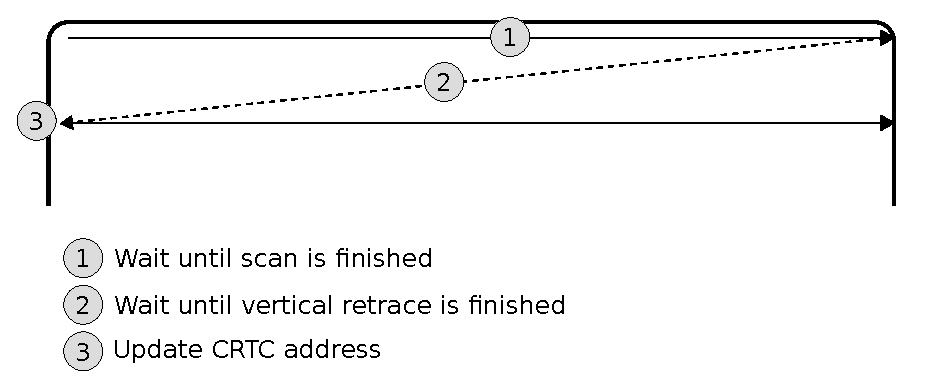
\includegraphics[width=\textwidth]{imgs/drawings/update_start_address.eps}
  \label{fig:update_start_address}
  \caption{Update CRTC start address at beginning of new scan line.}
\end{figure}

\par
To guarantee that the start address updates at the very beginning of a new scan line, the process first waits until the current scan line completes. Then, it waits for a full retrace, checking that the Display Enable Status returns to '0'. At this point, the CRTC address is updated.\\

\trivia{Regardless of CPU speed, the game's speed is limited by the CRTC sync to the monitor's refresh rate, which is 60Hz for EGA and 70Hz for VGA.}

\par
\begin{minipage}{\textwidth}
\lstinputlisting[language={[x86masm]Assembler}]{code/screen_refresh.c}
\end{minipage}
\par

\subsection{Manage Refresh Timing}
After each screen refresh, a certain amount of time, referred to as "ticks", has passed. The tick count depends on several factors, such as the number of tiles refreshed and the waiting period for a screen's vertical retrace. Since all game actions and reactions rely on the tick interval between two refreshes, it is important to keep this interval consistent.\\

\par
Without controlling the tick interval, the state and speed of actors can become unpredictable, potentially causing them to move too quickly or even "warp" to an unexpected location. To manage refresh intervals effectively, a minimum and maximum number of ticks are defined within the refresh loop.\\

\par
\begin{minipage}{\textwidth}
  \lstinputlisting[language=C]{code/time_ticks.c}
\end{minipage}
\label{time_ticks}

\pagebreak
\section{Actors and AI}
\label{section:actors_and_ai}

\subsection{State Machine}
All objects in the game, such as Commander Keen, enemies, bonus points, doors, and even the scoreboard, are called "actors". Each actor can "think" and perform actions like walking, shooting, or emitting sounds. Actors are controlled via a state machine, enabling them to take actions such as chasing the player, running in various directions, throwing objects, or doing nothing at all. To model their behavior, all enemies have an associated state, which can include:
\begin{itemize}
  \item Chasing Keen
  \item Hitting or smashing Keen
  \item Shooting projectiles
  \item Climbing and sliding on poles
  \item Turning into a flower
  \item Special Boss (Boobus)
\end{itemize}

\par
Each state has associated think, reaction, and contact method pointers. Additionally, there is a \cw{tictime} and \cw{*nextstate} pointer, which indicate when the actor should transition to another state after a specific number of tics have passed in the current state.\\

\par
\begin{minipage}{\textwidth}
  \lstinputlisting[language=C]{code/statetype.c}
\end{minipage}
\label{state_type}
\par

Each actor has a defined state chain, as example the pea pod. \\
\par
\begin{minipage}{\textwidth}
\lstinputlisting[language=C,style=mystyle,basicstyle=\small]{code/s_grdchase.c}
\end{minipage}

\par
Different types of enemies have their own state machines, often sharing reaction function (e.g., WalkReact and ProjectileReact) but usually possessing their own unique "thinking" states.\\

\begin{figure}[H]
  \centering
  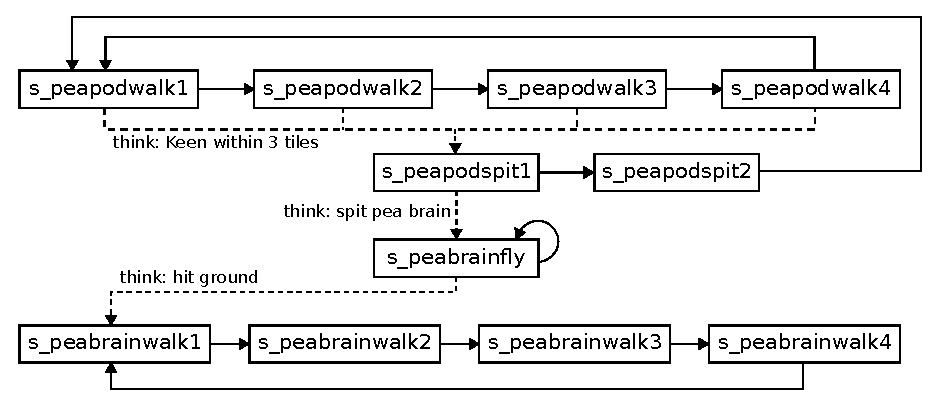
\includegraphics[width=\textwidth]{imgs/drawings/state_machine.eps}
  \caption{State machine for Pea pod and Pea brain.}
  \label{fig:state_machine}  
\end{figure}

\par
The \cw{*react} function is responsible for managing how an enemy reacts to the level, like turning around upon hitting a wall or the edge of a platform. The \cw{*think} function defines how an enemy behaves when Commander Keen is nearby (e.g., attacking or firing a projectile) or when it reaches an edge (e.g. jumping). In some cases it introduces randomness, like when a pea pod might decide to spit a pea brain.\\

\par
\begin{minipage}{\textwidth}
  \lstinputlisting[language=C]{code/state_machine_think.c}
\end{minipage}
\label{state_type}

\par
The \cw{*contact} function checks if an object has come into contact with another object and defines the resulting interaction, such as Commander Keen taking damage or losing a life.



\subsection{Clipping}
\label{section:clipping}
Whether an actor can move or fall through a tile is determined by the \cw{tinf[]} parameters. Each foreground tile includes four directional parameters: north, south, east, and west. If, for example, the east parameter has a value greater than 0, the tile is considered solid, and the actor cannot enter it from the east side. When a sprite moves to the left and encounters a solid tile from the east, the engine adjusts the actor's movement to prevent it from entering the tile.\\


\begin{figure}[H]
  \centering
  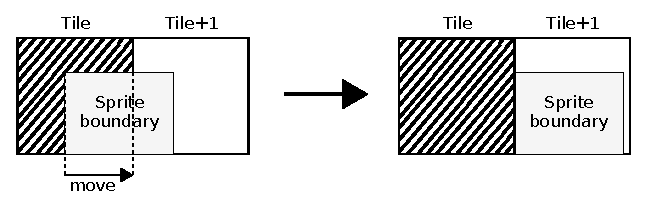
\includegraphics[width=\textwidth]{imgs/drawings/clipping_east.eps}
  \caption{Clipping to east wall when actor moves left.}
  \label{fig:clipping_east}  
\end{figure}

\par
\begin{minipage}{\textwidth}
  \lstinputlisting[language=C]{code/clip_east_wall.c}
\end{minipage}
\label{wallclip_array}
\par
For clipping along the top and bottom of tiles, the engine also accounts for standing on slopes. After the actor is clipped to the top or bottom of a slope tile, an offset is applied to move the actor up or down along the slope. \\

\begin{figure}[H]
  \centering
  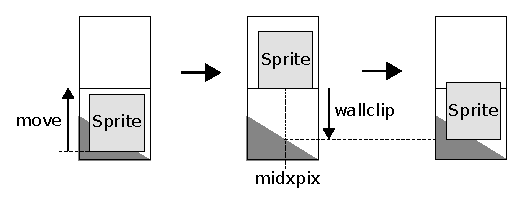
\includegraphics[width=\textwidth]{imgs/drawings/clipping_north.eps}
  \label{fig:clipping_north}
  \caption{Clipping north wall with slope.}
\end{figure}

This offset is defined by the lookup table \cw{wallclip[8][16]}, which uses the actor's midpoint and the wall type to determine the slope type.

\par
\begin{figure}[H]
  \centering
  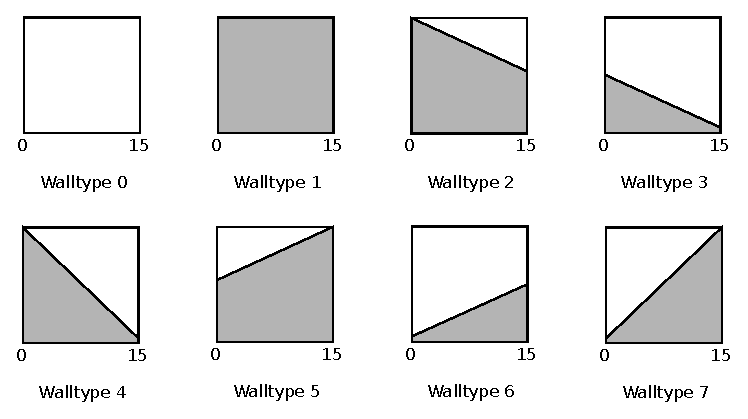
\includegraphics[width=\textwidth]{imgs/drawings/walltype.eps}
  \caption{Fall through, solid and 6 slope types.}
  \label{fig:walltype}
\end{figure}



\par
\begin{minipage}{\textwidth}
  \lstinputlisting[language=C]{code/clip_north_wall.c}
\end{minipage}
\label{wallclip_array}


\section{Drawing layer for layer}
Each tile on the screen can contain up to three layers: the background layer, the foreground layer and a sprite layer. Rendering the final screen requires multiple redraws on the same tile to achieve the correct layering:
\begin{enumerate}
  \item Draw the background layer or a combined background and foreground tile.
  \item Draw the sprites.
  \item Re-draw the foreground layer if a sprite should not appear on top.
\end{enumerate}

\par
It must run quickly and therefore most of the code is written in assembly.

\subsection{Draw background and foreground tiles}
Drawing the background layer is straightforward, as it only requires copying 128 bytes to VRAM. Drawing foreground tiles on top of the background layer requires an additional mask, which defines which pixels are overwritten by the foreground tile.\\

\begin{figure}[H]
\centering
 \begin{subfigure}{0.32\textwidth}
 	\centering
 	
\includegraphics[width=0.45\textwidth]{screenshots_300dpi/game/mask_tiles_1.png}
 	\caption{Background tile.}
 \end{subfigure}
 \begin{subfigure}{0.32\textwidth}
 	\centering
 	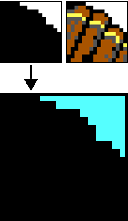
\includegraphics[width=0.45\textwidth]{screenshots_300dpi/game/mask_tiles_2.png}
 	\caption{\cw{AND} foreground mask.}
 \end{subfigure}
 \begin{subfigure}{0.32\textwidth}
 	\centering
 	
\includegraphics[width=0.45\textwidth]{screenshots_300dpi/game/mask_tiles_3.png}
 	\caption{\cw{OR} foreground bitmap.}
 \end{subfigure} 

\caption{Draw masked foreground tile.}
\label{fig:foreground_tile}
\end{figure}

Combining the background and foreground layers involves an \cw{AND}-bitwise operator to clear the background and the \cw{OR}-bitwise operator to write the foreground layer.\\

\par
\begin{minipage}{\textwidth}
  \lstinputlisting[language={[x86masm]Assembler}]{code/update_tile.asm}
  \end{minipage}
  \label{update_tile}


\subsection{Drawing sprites}
The next step is to render sprites on the screen. Most home computers of that era had built-in sprite functionality on the video card. For example, on a MSX computer, one could simply enter\\

\par
\begin{minipage}{\textwidth}
  \lstinputlisting[language=C]{code/msx_sprite.c}
  \end{minipage}
  \label{msx_sprite}

\par
to display a sprite on the screen. Updating the \cw{(X, Y)} coordinates would move the sprite, with the display adapter handling everything else. Unfortunately, the concept of sprites did not exist on EGA cards, so game developers had to implement their own solution.\\

\par
A challenge arises from the fact that sprites can move freely across the screen and are not byte-aligned. To address this, the bit-shifting technique described in section \ref{section:bitshifting} is used. When caching a sprite into memory, each sprite is copied four times, with each copy shifted by two or more pixels using this technique. The property \cw{*spr->shifts} determines the number of bit shifts applied to each of the four copies.\\


\begin{figure}[H]
  \centering
  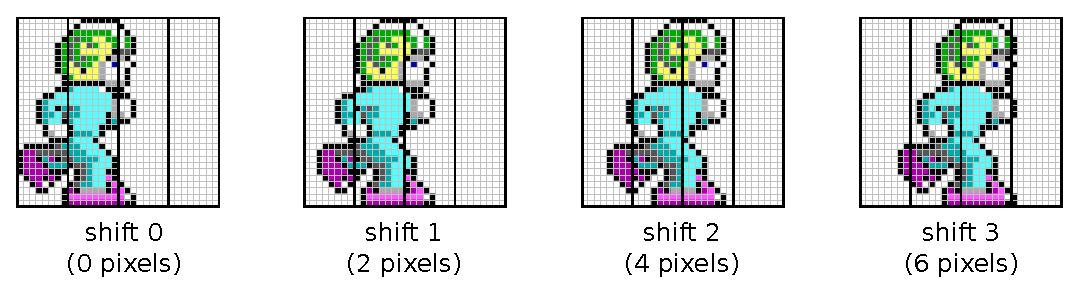
\includegraphics[width=\textwidth]{imgs/drawings/sprite_shift.eps}
  \caption{Sprite shifted in 4 steps.}
  \label{fig:sprite_shift}  
\end{figure}

\par
Displaying the correct shifted sprite is as simple as\\
\par
\begin{minipage}{\textwidth}
  \lstinputlisting[language=C]{code/sprite_shift.c}
  \end{minipage}
  \label{sprite_shift}  

\par
\begin{minipage}{\textwidth}
  \lstinputlisting[language=C]{code/shift_sprite.c}
  \end{minipage}
  \label{shift_sprite}
  

\par
If multiple sprites are displayed on the same tile, each sprite is assigned a priority from 0 to 3 to determine the drawing order. A sprite with a higher priority number is always drawn on top of sprites with a lower priority. Since sprites are always drawn on top of tiles, this can create unnatural situations, such as when Commander Keen is climbing through a hole, as illustrated in Figure \ref{fig:draw_layers}.\\

\begin{figure}[H]
\begin{subfigure}{.25\textwidth}
  \centering
  
\includegraphics[width=.9\textwidth]{screenshots_300dpi/game/tile_composite_1.png}
  \caption{Background tile.}
\end{subfigure}%
\begin{subfigure}{.25\textwidth}
  \centering
  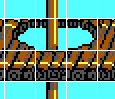
\includegraphics[width=.9\textwidth]{screenshots_300dpi/game/tile_composite_2.png}
  \caption{Foreground tile.}
\end{subfigure}
\begin{subfigure}{.25\textwidth}
  \centering
  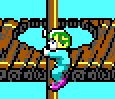
\includegraphics[width=.9\textwidth]{screenshots_300dpi/game/tile_composite_3.png}
  \caption{Sprite on top.}
\end{subfigure}
\caption{Unnatural situation where Commander Keen is in front of a hole.}
\label{fig:draw_layers}
\end{figure}

\par
To draw sprites 'inside' a foreground tile, a trick is used by introducing a priority foreground tile in the \cw{tinf} info table. The attribute is named INTILE ("in-front"). If a foreground tile has its INTILE attribute high bit set (\cw{80h}), sprites with priority 0-2 will not be drawn over it. Only sprites with priority 3 are drawn over the foreground tile. This results in the following drawing order:
\begin{enumerate}
  \item Draw the background tile and the masked foreground tile.
  \item Draw sprites with priority 0, 1, and 2 (in that order), and mark the corresponding tile in the tile buffer array with a '3', as illustrated in Figure \ref{fig:kc1_3_tile_update_sprite} on page \pageref{fig:kc1_3_tile_update_sprite}.
  \item Scan the tile buffer array for tiles marked with '3'. If the corresponding foreground tile's INTILE attribute high bit (\cw{80h}) is set, re-draw the foreground tile. 
  \item Finally, draw sprites with priority 3. These sprites are always drawn on top of everything.
\end{enumerate}
\par


\begin{figure}[H]
\centering
\begin{subfigure}[t]{.245\textwidth}
  \centering
  
\includegraphics[width=.9\textwidth]{screenshots_300dpi/game/tile_composite_1.png}
  \caption{Background tile.}
\end{subfigure}%
\begin{subfigure}[t]{.245\textwidth}
  \centering
  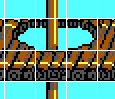
\includegraphics[width=.9\textwidth]{screenshots_300dpi/game/tile_composite_2.png}
  \caption{Foreground tile.}
\end{subfigure}
\begin{subfigure}[t]{.245\textwidth}
  \centering
  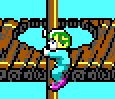
\includegraphics[width=.9\textwidth]{screenshots_300dpi/game/tile_composite_3.png}
  \caption{Sprite on top.}
\end{subfigure}
\begin{subfigure}[t]{.245\textwidth}
  \centering
  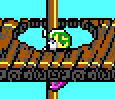
\includegraphics[width=.9\textwidth]{screenshots_300dpi/game/tile_composite_4.png}
  \caption{Redraw foreground tile.}
\end{subfigure}
\caption{Draw sprite inside a tile, by redrawing foreground tile.}
\label{fig:clip_tinf}
\end{figure}

\par
\begin{minipage}{\textwidth}
  \lstinputlisting[language={[x86masm]Assembler}]{code/mask_foreground_tile.asm}
\end{minipage}
\label{mask_foreground_tile}
\par

\subsection{Tile Draw Performance Tricks}
To draw one background tile to VRAM, the engine must read and write 128 bytes (2 x 16 bytes x 4 memory banks), which is the minimum number of read/write operations required. In the worst case, up to 512 bytes of read/write operations are required (background, foreground, sprite, and foreground again), with multiple bitwise operations involved.
The engine employs several tricks to squeeze the maximum out of each CPU cycle: background tile caching and word-aligned memory writing.

\subsubsection{Background Tile Caching}
When updating the master screen in VRAM, the engine copies each tile from RAM to VRAM. Copying each pixel involves one read and one write operation across the four memory banks. As explained in section \ref{section:optimize_tile}, by reprogramming the latches on the EGA card, it is possible to copy four bytes at once from one VRAM location to another. The same technique can be applied to tiles containing only a background layer.\\

\par
Once a background tile is loaded into the master screen, subsequent requests for the same tile can be handled by copying it directly from VRAM using the reprogrammed latches, rather than copying from RAM. The engine only needs to track which background tiles are already loaded into VRAM using an array.\\

\par
\begin{minipage}{\textwidth}
  \lstinputlisting[language=C]{code/tile_cache.c}
\end{minipage}

\par
The assembly function \cw{RFL\_NewTile} is responsible for drawing tiles to the master screen. It first checks whether the background tile is already stored in the tile cache array. If it is, the tile is copied at 32 bits per cycle from VRAM to VRAM. Otherwise, the tile is loaded from RAM, and the VRAM pointer for that tile is stored in the tile cache array for future use.\\

\par
\begin{minipage}{\textwidth}
  \lstinputlisting[language={[x86masm]Assembler}]{code/RFL_NewTile.ASM}
\end{minipage}
\par

\subsubsection{Word-aligned memory writing}
The 286 CPU can read and write 16 bits in a single cycle, but there is a caveat: this only works when accessing even memory addresses. Additionally, writing a word at the offset address \cw{FFFFh} causes an exception.\\

\par
Because tiles are word-aligned (16 bits wide) and the screen refreshes in tile-sized steps, they are always aligned with even memory addresses. However, sprites are byte-aligned. When a sprite is drawn from an odd memory address, the CPU is limited to reading and writing 8 bits at a time. To fully utilize the 16-bit data bus, the engine uses small function routines for each combination of sprite width and even/odd address alignment.\\

\begin{figure}[H]
  \centering
  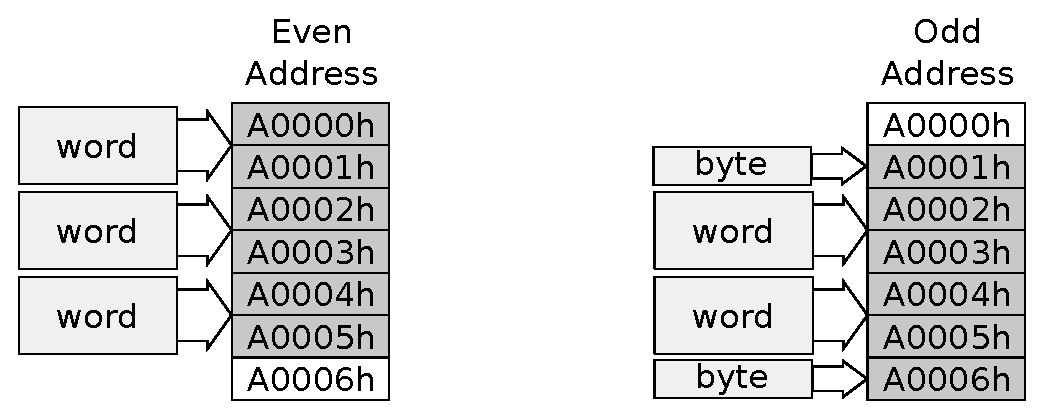
\includegraphics[width=0.75\textwidth]{imgs/drawings/mask_block.eps}
  \caption{Word-optimized 6 byte wide sprite to even (\cw{MASK6E}) and odd (\cw{MASK6O}) address.}
  \label{fig:mask_block}  
\end{figure}

\par
In total 23 functions are written to optimize \cw{word}-size writing up to 10 bytes wide sprites. Each function pointer reference is stored in an array.\\

\par
\begin{minipage}{\textwidth}
  \lstinputlisting[language={[x86masm]Assembler}]{code/VW_maskroutines.asm}
\end{minipage}

\par
The engine first determines whether the destination is at an even or odd memory address. If the address is odd, it first writes a single byte to align the subsequent operations to an even address, after which it continues writing in 16-bit words. 
By cleverly using bit-shift operations and the Carry Flag (CF), the engine calls the appropriate function to write the sprite to VRAM.\\

\par
\begin{minipage}{\textwidth}
  \lstinputlisting[language={[x86masm]Assembler}]{code/VW_MaskBlock.asm}
\end{minipage}
\par





\end{document}